% Options for packages loaded elsewhere
\PassOptionsToPackage{unicode}{hyperref}
\PassOptionsToPackage{hyphens}{url}
%
\documentclass[
]{article}
\usepackage{lmodern}
\usepackage{amssymb,amsmath}
\usepackage{ifxetex,ifluatex}
\ifnum 0\ifxetex 1\fi\ifluatex 1\fi=0 % if pdftex
  \usepackage[T1]{fontenc}
  \usepackage[utf8]{inputenc}
  \usepackage{textcomp} % provide euro and other symbols
\else % if luatex or xetex
  \usepackage{unicode-math}
  \defaultfontfeatures{Scale=MatchLowercase}
  \defaultfontfeatures[\rmfamily]{Ligatures=TeX,Scale=1}
\fi
% Use upquote if available, for straight quotes in verbatim environments
\IfFileExists{upquote.sty}{\usepackage{upquote}}{}
\IfFileExists{microtype.sty}{% use microtype if available
  \usepackage[]{microtype}
  \UseMicrotypeSet[protrusion]{basicmath} % disable protrusion for tt fonts
}{}
\makeatletter
\@ifundefined{KOMAClassName}{% if non-KOMA class
  \IfFileExists{parskip.sty}{%
    \usepackage{parskip}
  }{% else
    \setlength{\parindent}{0pt}
    \setlength{\parskip}{6pt plus 2pt minus 1pt}}
}{% if KOMA class
  \KOMAoptions{parskip=half}}
\makeatother
\usepackage{xcolor}
\IfFileExists{xurl.sty}{\usepackage{xurl}}{} % add URL line breaks if available
\IfFileExists{bookmark.sty}{\usepackage{bookmark}}{\usepackage{hyperref}}
\hypersetup{
  pdftitle={Methods to prioritise pop-up active transport infrastructure and their application in a national cycleway prioritisation tool},
  pdfauthor={Robin Lovelace, Joey Talbot, Malcolm Morgan, Martin-Lucas-Smith},
  hidelinks,
  pdfcreator={LaTeX via pandoc}}
\urlstyle{same} % disable monospaced font for URLs
\usepackage[margin=1in]{geometry}
\usepackage{longtable,booktabs}
% Correct order of tables after \paragraph or \subparagraph
\usepackage{etoolbox}
\makeatletter
\patchcmd\longtable{\par}{\if@noskipsec\mbox{}\fi\par}{}{}
\makeatother
% Allow footnotes in longtable head/foot
\IfFileExists{footnotehyper.sty}{\usepackage{footnotehyper}}{\usepackage{footnote}}
\makesavenoteenv{longtable}
\usepackage{graphicx}
\makeatletter
\def\maxwidth{\ifdim\Gin@nat@width>\linewidth\linewidth\else\Gin@nat@width\fi}
\def\maxheight{\ifdim\Gin@nat@height>\textheight\textheight\else\Gin@nat@height\fi}
\makeatother
% Scale images if necessary, so that they will not overflow the page
% margins by default, and it is still possible to overwrite the defaults
% using explicit options in \includegraphics[width, height, ...]{}
\setkeys{Gin}{width=\maxwidth,height=\maxheight,keepaspectratio}
% Set default figure placement to htbp
\makeatletter
\def\fps@figure{htbp}
\makeatother
\setlength{\emergencystretch}{3em} % prevent overfull lines
\providecommand{\tightlist}{%
  \setlength{\itemsep}{0pt}\setlength{\parskip}{0pt}}
\setcounter{secnumdepth}{5}
\usepackage{booktabs}
\usepackage{longtable}
\usepackage{array}
\usepackage{multirow}
\usepackage{wrapfig}
\usepackage{float}
\usepackage{colortbl}
\usepackage{pdflscape}
\usepackage{tabu}
\usepackage{threeparttable}
\usepackage{threeparttablex}
\usepackage[normalem]{ulem}
\usepackage{makecell}
\usepackage{xcolor}
\newlength{\cslhangindent}
\setlength{\cslhangindent}{1.5em}
\newenvironment{cslreferences}%
  {\setlength{\parindent}{0pt}%
  \everypar{\setlength{\hangindent}{\cslhangindent}}\ignorespaces}%
  {\par}

\title{Methods to prioritise pop-up active transport infrastructure and their application in a national cycleway prioritisation tool}
\author{Robin Lovelace, Joey Talbot, Malcolm Morgan, Martin-Lucas-Smith}
\date{}

\begin{document}
\maketitle

{
\setcounter{tocdepth}{2}
\tableofcontents
}
\hypertarget{abstract}{%
\section{Abstract}\label{abstract}}

In the context of reduced public transport capacity in the wake of the COVID-19 pandemic, governments are scrambling to enable walking and cycling while adhering to physical distancing guidelines.
A range of pop-up options exist, include road space reallocation, which represents a `quick win' for cities with `spare space' along continuous road sections that have high latent cycling potential.
We developed methods to condense the complexity of city networks down to the most promising roads for road space reallocation schemes.
The resulting Rapid Cycleway Prioritisation Tool has been deployed for all local and regional transport authorities in England to help prioritise emergency funds for new cycleways nationwide.
The approach could be used to support investment in pop-up infrastructure in cities worldwide.

\hypertarget{research-questions-and-hypothesis}{%
\section{RESEARCH QUESTIONS AND HYPOTHESIS}\label{research-questions-and-hypothesis}}

Much attention has focused on the impacts of COVID-19 on long-distance travel patterns (e.g.~Iacus et al. 2020; Jittrapirom and Tanaksaranond 2020) but short distance travel patterns have also changed.
There has been a notable increase in cycling in some areas (Harrabin 2020) due to the increased need for exercise close to home for mental and physical health (Jim\a'enez-Pav\a'on, Carbonell-Baeza, and Lavie 2020) and a reduction in public transport options (e.g.~Tian et al. 2020).
The second reason is particularly important given that many `key workers' are low paid, with limited access to private automobiles.

Local and national governments are working out how best to respond.
Many options are available to ensure that citizens can benefit from outdoor activity while minimising health risks, ranging from hand sanitiser provision to the creation of extra active transport space (Freeman and Eykelbosh 2020).
Installation of `pop-up' active transport infrastructure has been endorsed and implemented in many places (Laker 2020).
The Scottish government, for example, has provided £10 million ``to keep key workers moving'' by ``reallocating road space to better enable this shift and make it safer for people who choose to walk, cycle or wheel for essential trips or for exercise'' (Transport Scotland 2020).
On 9\textsuperscript{th} May 2020, the UK government announced a £250 million package for pop-up active transport infrastructure (Reid 2020).
Significantly, alongside this funding comes updated \href{https://www.gov.uk/government/publications/reallocating-road-space-in-response-to-covid-19-statutory-guidance-for-local-authorities/traffic-management-act-2004-network-management-in-response-to-covid-19}{statutory guidance} on pop-up infrastructure and safety.
Evidence is needed to ensure that such investment is spent effectively and where it is most needed.

Most pop-up active transport infrastructure can be classified into three broad categories:

\begin{enumerate}
\def\labelenumi{\arabic{enumi}.}
\tightlist
\item
  Measures such as point closures or contraflow cycle lanes, which can be used to promote `filtered permeability', a strategy in which street networks are redesigned so that routes for cyclists are faster and more direct than routes for drivers. An example of this is \href{https://twitter.com/TowerHamletsNow/status/1257564043856019458}{shown} in {[}Tower Hamlets{]}.
\item
  Measures to close roads entirely to cars, either permanently or at certain times of day, as in New York's `Open Streets' scheme (Litman 2020).
\item
  Measures to reallocate space on wide roads to create new cycleways or to widen pavements (Orsman 2020).
\end{enumerate}

The focus of this article is on the third category.
The research question is:

\begin{quote}
How can automated data analysis and interactive visualisation methods help prioritise the reallocation of road space for pop-up active transport infrastructure?
\end{quote}

Because of the recent, localised and often ad-hoc nature of pop-up infrastructure, it is difficult to make, let alone test, hypotheses related to the research question.
Our broad hypothesis is that digital tools based on open data, combined with crowdsourcing such as the interactive map used to support community-level responses to COVID-19 in Salford (Salford City Council 2020), illustrated in Figure 1, can lead to more effective use of resources allocated to pop-up interventions.

\begin{figure}
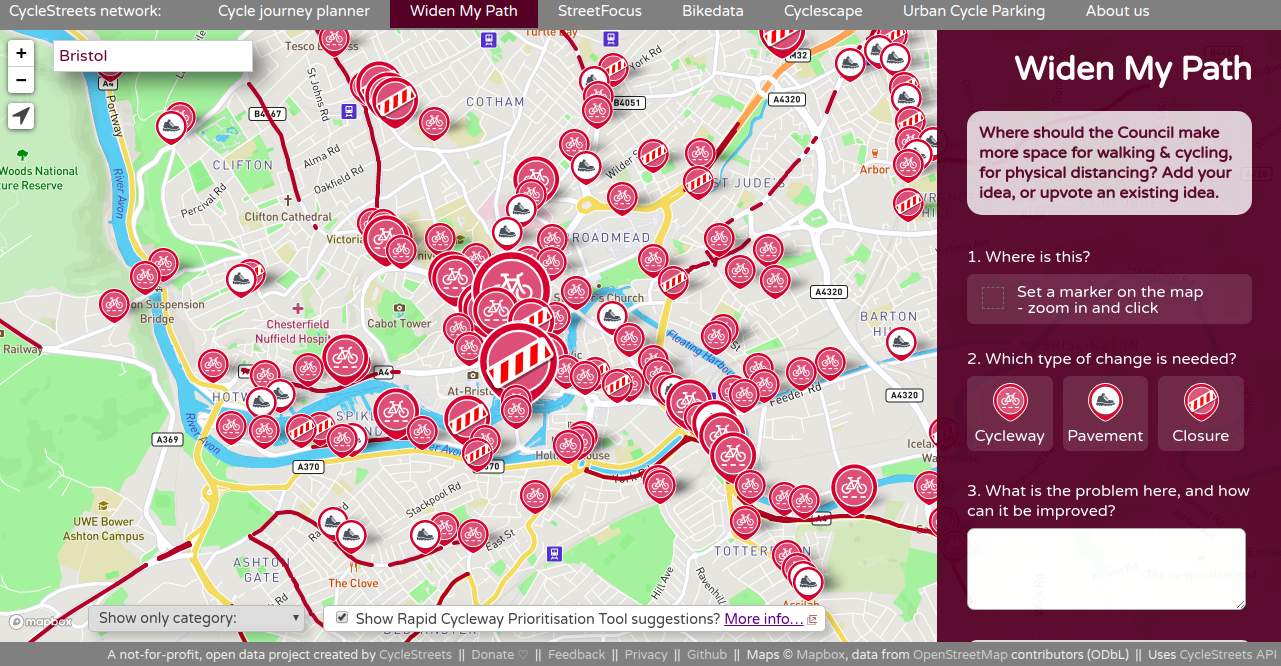
\includegraphics[width=1\linewidth]{figures/widenmypath} 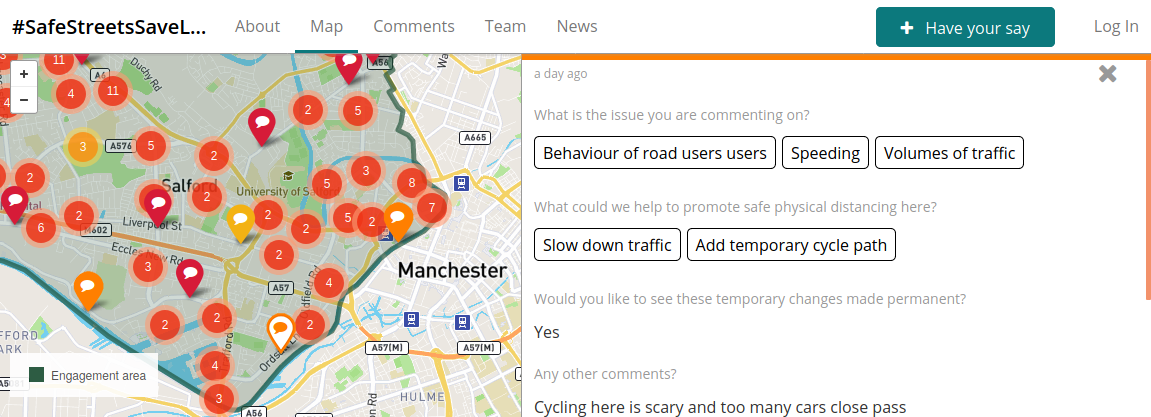
\includegraphics[width=1\linewidth]{figures/saferstreets} \caption{Screenshots from the websites widenmypath.com (top) which includes top cycle route recommendations generated using the methods outlined in this paper in an open web forum, and salfordliveablestreets.commonplace.is (bottom) to support local responses to the COVID-19 pandemic, including the prioritisation of pop-up active transport infrastructure.}\label{fig:commonplace}
\end{figure}

\hypertarget{methods-and-data}{%
\section{METHODS AND DATA}\label{methods-and-data}}

Two key datasets were used for the project:

\begin{itemize}
\tightlist
\item
  Estimates of cycling potential at the street segment level from the UK Department for Transport funded Propensity to Cycle Tool (PCT) project (Goodman et al. 2019; Lovelace et al. 2017)
\item
  Data derived from OpenStreetMap, with several new variables added to support cycling infrastructure planning (see www.cyipt.bike for an overview)
\end{itemize}

Datasets from the PCT and CyIPT project were merged, resulting in crucial variables summarised in Table 1.
Cycling potential is defined as the number of one-way journeys to work and to school, under a scenario in which the government aim of doubling cycling levels is met.
This does not include other types of journey such as leisure and shopping.

Roads are classified by speed limit because this has been shown to be a key factor associated with the incidence of severe injuries and fatalities of cyclists (Chen and Shen 2016), with odds of cyclist injury on 20 mph (32.2 kmph) roads in London found to be 21\% lower than on 30 mph (48.3 kmph) roads (Aldred et al. 2018).
Therefore the suitability of roads for cycle infrastructure, the preferred degree of physical segregation, or the necessity to reduce traffic speeds could all be influenced by current speed limits.

\begin{table}

\caption{\label{tab:t1}Summary of the road segment dataset for Leeds. Units of speed are in miles per hour (mph), with 20, 30 and 40 mph representing 32, 48 and 64 kilometers per hour respectively.}
\centering
\begin{tabular}[t]{lllll}
\toprule
 & 20 mph or less & 30 mph & 40+ mph & Overall\\
\midrule
\addlinespace[0.3em]
\multicolumn{5}{l}{\textbf{N. observations}}\\
\hspace{1em} & 4777 & 19241 & 3105 & 27123\\
\addlinespace[0.3em]
\multicolumn{5}{l}{\textbf{Highway type}}\\
\hspace{1em}\hspace{1em}bridleway & 53 (1.1\%) & 0 (0\%) & 0 (0\%) & 53 (0.2\%)\\
\hspace{1em}cycleway & 1214 (25.4\%) & 0 (0\%) & 0 (0\%) & 1214 (4.5\%)\\
\hspace{1em}footway & 1332 (27.9\%) & 0 (0\%) & 0 (0\%) & 1332 (4.9\%)\\
\hspace{1em}other & 187 (3.9\%) & 715 (3.7\%) & 1608 (51.8\%) & 2510 (9.3\%)\\
\hspace{1em}pedestrian/living\_street & 22 (0.5\%) & 0 (0\%) & 0 (0\%) & 22 (0.1\%)\\
\hspace{1em}primary & 14 (0.3\%) & 1432 (7.4\%) & 955 (30.8\%) & 2401 (8.9\%)\\
\hspace{1em}residential & 605 (12.7\%) & 8604 (44.7\%) & 0 (0\%) & 9209 (34.0\%)\\
\hspace{1em}secondary & 28 (0.6\%) & 1408 (7.3\%) & 176 (5.7\%) & 1612 (5.9\%)\\
\hspace{1em}service & 1018 (21.3\%) & 7 (0.0\%) & 0 (0\%) & 1025 (3.8\%)\\
\hspace{1em}tertiary & 170 (3.6\%) & 5206 (27.1\%) & 290 (9.3\%) & 5666 (20.9\%)\\
\hspace{1em}unclassified & 134 (2.8\%) & 1869 (9.7\%) & 75 (2.4\%) & 2078 (7.7\%)\\
\hspace{1em}bus\_guideway & 0 (0\%) & 0 (0\%) & 1 (0.0\%) & 1 (0.0\%)\\
\addlinespace[0.3em]
\multicolumn{5}{l}{\textbf{Cycling potential}}\\
\hspace{1em}Mean (SD) & 39.0 (67.8) & 36.9 (66.7) & 40.7 (55.1) & 37.7 (65.7)\\
\hspace{1em}Median [Min, Max] & 14.0 [1.00, 810] & 15.0 [1.00, 810] & 24.0 [1.00, 519] & 16.0 [1.00, 810]\\
\addlinespace[0.3em]
\multicolumn{5}{l}{\textbf{Width (m)}}\\
\hspace{1em}Mean (SD) & 6.62 (2.71) & 7.34 (2.28) & 8.84 (2.36) & 7.41 (2.42)\\
\hspace{1em}Median [Min, Max] & 7.00 [1.00, 21.0] & 7.00 [1.00, 24.0] & 9.00 [2.00, 21.0] & 7.00 [1.00, 24.0]\\
\hspace{1em}Missing & 1688 (35.3\%) & 1225 (6.4\%) & 447 (14.4\%) & 3360 (12.4\%)\\
\addlinespace[0.3em]
\multicolumn{5}{l}{\textbf{N. lanes}}\\
\hspace{1em}1 & 3840 (80.4\%) & 1555 (8.1\%) & 406 (13.1\%) & 5801 (21.4\%)\\
\hspace{1em}2 & 937 (19.6\%) & 16979 (88.2\%) & 2266 (73.0\%) & 20182 (74.4\%)\\
\hspace{1em}3 & 0 (0\%) & 490 (2.5\%) & 289 (9.3\%) & 779 (2.9\%)\\
\hspace{1em}4+ & 0 (0\%) & 217 (1.1\%) & 144 (4.6\%) & 361 (1.3\%)\\
\bottomrule
\end{tabular}
\end{table}

\hypertarget{geographic-subsetting}{%
\subsection{Geographic subsetting}\label{geographic-subsetting}}

The region of analysis may seem like a basic consideration: most cities have well-defined administrative zones.
In Leeds and many other cities, it makes sense to focus on the region directly surrounding the city centre, in a kind of `geographical triage' to omit from the analysis pop-up options in the outskirts, focus valuable attention on the routes that are most likely to serve the highest number of people, and ensure that road sections outside administrative areas but close to key destinations are included.

Figure \ref{fig:gsub} shows three broad strategies for geographic subsetting: based on administrative boundaries, distance from the centre, and distance from the centre and key destinations.
Major hospitals are used to illustrate the third strategy, as many key workers need to get to hospitals.
Schools could also be used here as an example of a key destination that may not fit well within administrative zones.
The latter case (Figure \ref{fig:gsub}, right) shows that administrative boundaries can exclude important roads.
The definition of `city centres' and `key destinations' is straightforward in clearly defined and well-understood city planning contexts.
In contexts where the method must be deployed nationwide, however the use of such subsetting approaches was found to be problematic, so the Rapid Cycleway Prioritisation Tool for England (v1) uses the first subsetting option, but subsets by larger regional boundaries to encourage regional collaboration on cycleway network design.

\begin{figure}
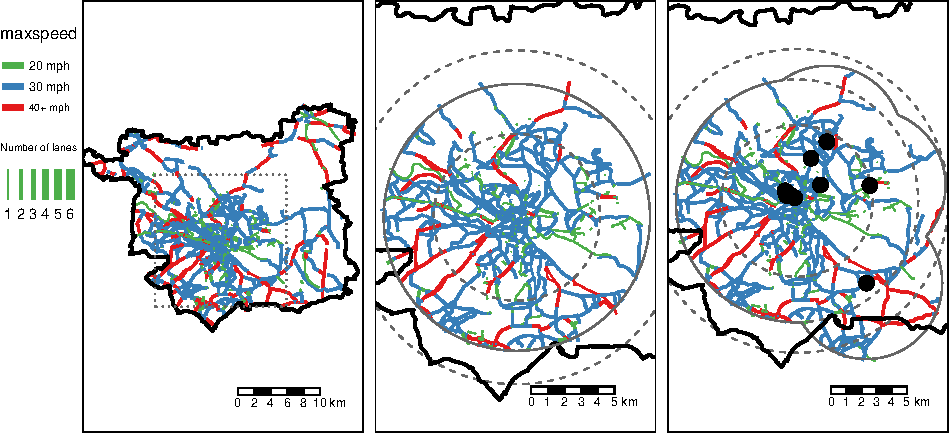
\includegraphics[width=1\linewidth]{article_files/figure-latex/gsub-1} \caption{Illustration of geographic subsetting based on administrative boundaries (left), distance to a central point (middle) and distance to city centre or key destinations (right). Radii of 5 km, 8 km and 10 km are shown for reference (note that some roads within 10 km of the center are outside the regional boundary). Units of speed are in miles per hour (mph), with 20, 30 and 40 mph representing 32, 48 and 64 kilometers per hour respectively.}\label{fig:gsub}
\end{figure}

\hypertarget{road-attributes}{%
\subsection{Road attributes}\label{road-attributes}}

Pop-up cycleways can be placed either on the side of wide roads (as is the case on \href{https://www.lancasterguardian.co.uk/news/uk-news/mixed-reactions-new-lancaster-pop-cycle-lanes-busy-city-centre-road-2875909}{South Road, Lancaster}) or in an entire lane that has been closed to motor traffic (as is the case on \href{https://metro.co.uk/2020/05/14/road-turns-giant-cycle-lane-make-social-distancing-easier-12703847/}{Park Lane}, London).
Accordingly, we defined `spare space' as either roads on which there is more than one lane in either direction or lane width above a threshold (set at 10 m based on feedback from engineers and the observation that South Road has a width of \textasciitilde9 m yet can just fit cycleways protected by plastic `wands').
This definition assumes no alteration of the navigable network for motor vehicles.

To identify road sections with a spare lane we developed a simple algorithm that takes the OSM variable \href{https://wiki.openstreetmap.org/wiki/Key:lanes}{\texttt{lanes}} if it is present and, if not, derives the number from the highway type and presence/absence of bus lanes.
Width estimates were taken from the CyIPT tool (see \href{https://www.cyipt.bike/}{www.cyipt.bike} for details).
All segments defined as having a spare space using this method are shown in Figure \ref{fig:levels} (left).

\hypertarget{attribute-filtering-and-grouping}{%
\subsection{Attribute filtering and grouping}\label{attribute-filtering-and-grouping}}

To ensure our route recommendations could achieve sufficient coherency, we undertook several stages of road segment filtering and grouping.
Segments were grouped by road reference number (i.e.~`A' or `B' road number) and by proximing, within a 100 m buffer.
Filtering then removed groups without distance weighted mean width \textgreater= 10 m or spare lanes along the majority of their length, and groups with distance-weighted mean cycling potential below a minimum threshold.

Segments without a reference number were subjected to stricter filtering criteria, to prevent the inclusion of unwanted short segments on side streets.
For all segments, a final round of grouping (ignoring previous groups) with a 100 m buffer was then used to remove groups with length below 500 m.
This step removed short sections distant from any others, thus improving the coherency of the results.
Finally, road names were used to identify continuous road sections with the same name of length \textgreater= 500m.
Groups containing five or more different named roads were labeled ``Unnamed road.''
An example of the impact of grouping strategy is shown in Figure \ref{fig:levels}.
The resulting network shows that grouping the segments first then filtering based on mean group-level attributes results in a more cohesive network than filtering individual segments then grouping the results.

\begin{figure}
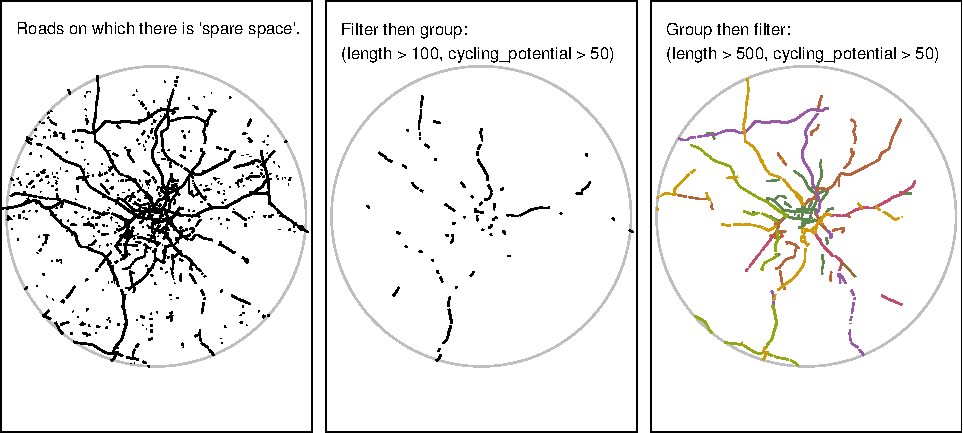
\includegraphics[width=1\linewidth]{article_files/figure-latex/levels-1} \caption{Illustration of the 'group then filter' method to identify roads with spare space that meet threshold values for length and cycling potential. The right hand panel contains roads on which the majority of segments have spare space (including segments that may not on their own be estimated to have spare space), coloured by group membership.}\label{fig:levels}
\end{figure}

\hypertarget{selection-of-top-routes}{%
\subsection{Selection of top routes}\label{selection-of-top-routes}}

Top routes were selected from the results of the previous steps.
These must not be labeled ``Unnamed road'' or have existing cycleways along more than 80\% of their length.
A high threshold was chosen here because the presence of an existing cycleway on OSM does not mean that this is necessarily a high quality cycleway.
Continuity of cycle provision is important for creating high quality networks (Parkin 2018).

\hypertarget{findings}{%
\section{FINDINGS}\label{findings}}

The results of the method applied to the city of Leeds are shown in Figure \ref{fig:res} (see \href{https://www.cyipt.bike/rapid/west-yorkshire/}{cyipt.bike/rapid} for interactive version) and Table 2.
We found that analysis of open transport network data, alongside careful selection of parameters, can generate plausible results for the prioritisation of pop-up cycle infrastructure.
Reducing the 85,000 road segments for Leeds down to a handful of candidate segments with more than 1 lane near key destinations has great potential to support policy-makers, especially when decisions need to be made fast.

\begin{figure}
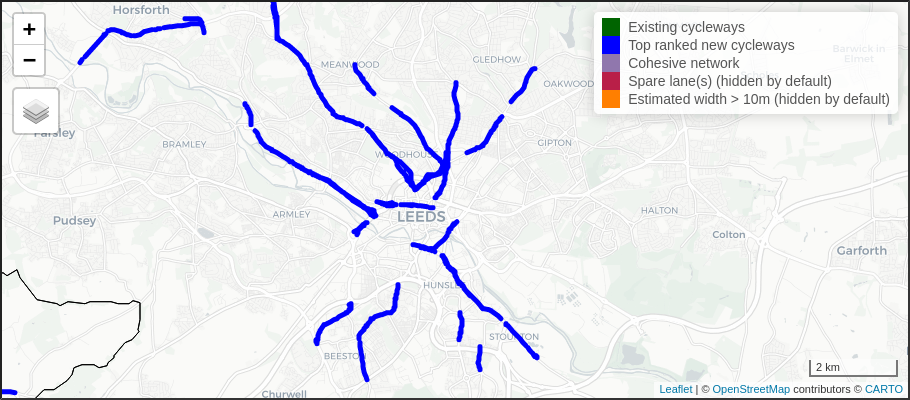
\includegraphics[width=1\linewidth]{figures/results-top-leeds} \caption{Results, showing road segments with a spare lane (light blue) and road groups with a minium threshold length, 1km in this case (dark blue). The top 10 road groups are labelled.}\label{fig:res}
\end{figure}

\begin{table}

\caption{\label{tab:unnamed-chunk-2}The top 10 candidate roads for space reallocation for pop-up lane reallocation interventions. Roads with 'spare lanes' identified using methods presented in the paper are ranked by cycling potential under the Government Target scenario, representing a doubling in commuter and school cycling levels compared with 2011 levels.}
\centering
\begin{tabular}[t]{lrrr}
\toprule
Name & Length (m) & Potential (Government Target) & Km/day (length * potential)\\
\midrule
Headingley Lane & 971 & 546 & 530\\
A660 & 718 & 414 & 297\\
Woodhouse Lane & 2438 & 372 & 907\\
A65 & 787 & 238 & 187\\
Kirkstall Road & 4407 & 237 & 1044\\
\addlinespace
Clay Pit Lane & 2235 & 231 & 516\\
Low Road & 516 & 194 & 100\\
Chapeltown Road & 1744 & 163 & 284\\
Roundhay Road & 909 & 161 & 146\\
Dewsbury Road & 538 & 157 & 84\\
\bottomrule
\end{tabular}
\end{table}

After initially developing the method for a single city, we applied the methods nationwide.
An illustration of the scale of the results is shown in Figure \ref{fig:facet}, which shows the results for six major cities in England, including existing cycleway and `cohesive network' layers, described on the tool's website \href{https://www.cyipt.bike/rapid/}{cyipt.bike/rapid}.
Local authorities are planning new pop-up cycleways informed by a range of sources of evidence, including the Rapid Cycleway Prioritisation Tool, and in many cases the plans match the routes highlighted by our tool.\footnote{
  \href{https://www.bbc.co.uk/news/uk-england-leeds-52577554}{Kirkstall Road} in Leeds and \href{https://www.se16.com/6208-work-starts-on-54m-cycleway-along-jamaica-road}{Jamaica Road} in London are a couple of examples.
  Many more examples can be found on posts mentioning the tool on \href{https://twitter.com/search?q=cyipt.bike\%2Frapid}{social media}.}

\begin{figure}
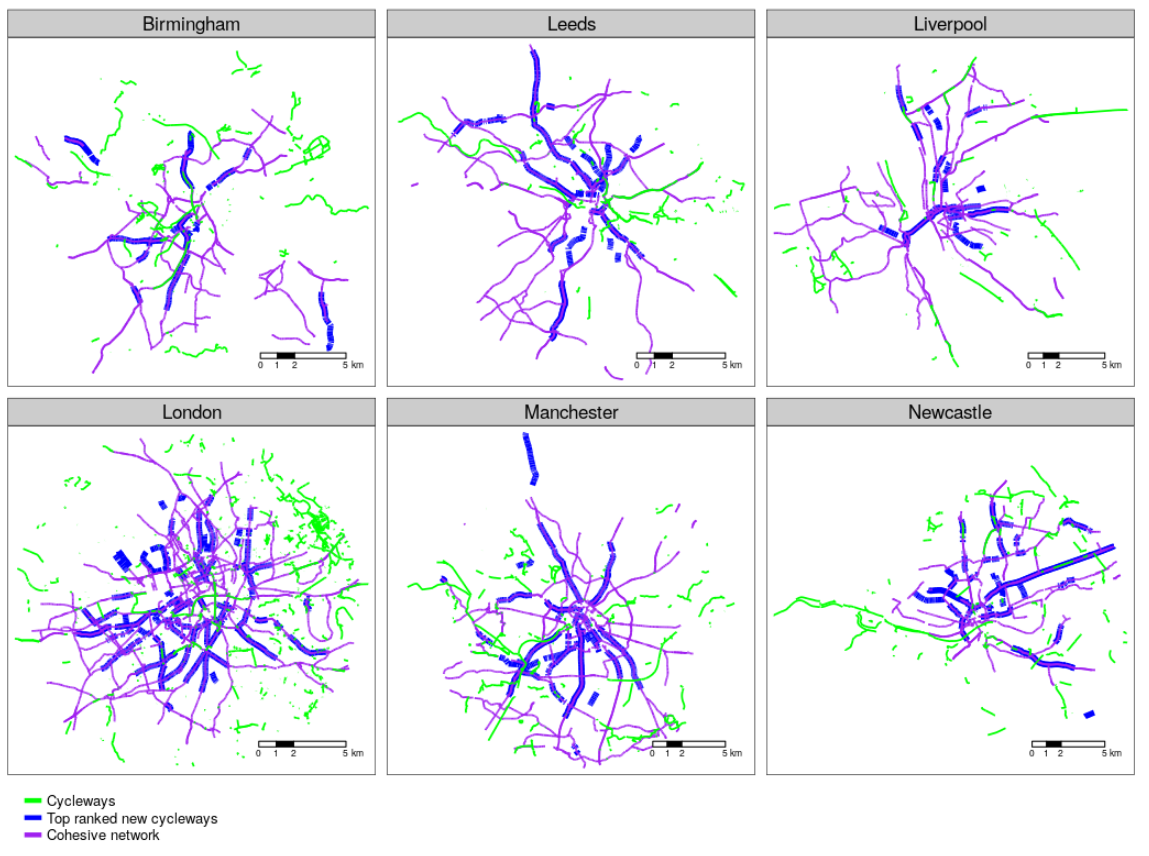
\includegraphics[width=1\linewidth]{figures/facet-output} \caption{Maps showing existing, disjointed cycleway networks (green), potential cycleway routes on wide roads according to the Rapid Cycleway Prioritisation Tool (blue) and cohesive networks (purple) in 6 major cities}\label{fig:facet}
\end{figure}

The approach is not without limitations.
Its reliance on data rather than community engagement represents a rather top-down approach to transport planning.
The incorporation of our results into participatory maps such as the one presented in Figure \ref{fig:commonplace} will help to mitigate this limitation.
Further work could also extend the method in various ways, for example by refining estimates of cycling potential based on additional parameters such as proximity to key destinations.
We welcome feedback on the results and methods at \href{https://github.com/cyipt/popupCycleways}{github.com/cyipt/popupCycleways}.

A major advantage of the approach is that it is scalable.
It would be feasible to internationalise the approach, given sufficient computer and developer resource to overcome the key data barriers: lack to cycling potential data and lack of road width data that are specific to the UK.
In summary, the methods presented can help lock-in the benefits of COVID-19 related cycling booms long term.

\hypertarget{references}{%
\section*{References}\label{references}}
\addcontentsline{toc}{section}{References}

\hypertarget{refs}{}
\begin{cslreferences}
\leavevmode\hypertarget{ref-aldred_cycling_2018}{}%
Aldred, Rachel, Anna Goodman, John Gulliver, and James Woodcock. 2018. ``Cycling Injury Risk in London: A Case-Control Study Exploring the Impact of Cycle Volumes, Motor Vehicle Volumes, and Road Characteristics Including Speed Limits.'' \emph{Accident Analysis \& Prevention} 117 (August): 75--84. \url{https://doi.org/10.1016/j.aap.2018.03.003}.

\leavevmode\hypertarget{ref-chen_built_2016}{}%
Chen, Peng, and Qing Shen. 2016. ``Built Environment Effects on Cyclist Injury Severity in Automobile-Involved Bicycle Crashes.'' \emph{Accident Analysis \& Prevention} 86: 239--46.

\leavevmode\hypertarget{ref-freeman_covid19_2020}{}%
Freeman, Shirra, and Angela Eykelbosh. 2020. ``COVID-19 and Outdoor Safety: Considerations for Use of Outdoor Recreational Spaces.'' BC Centre for Disease Control.

\leavevmode\hypertarget{ref-goodman_scenarios_2019}{}%
Goodman, Anna, Ilan Fridman Rojas, James Woodcock, Rachel Aldred, Nikolai Berkoff, Malcolm Morgan, Ali Abbas, and Robin Lovelace. 2019. ``Scenarios of Cycling to School in England, and Associated Health and Carbon Impacts: Application of the `Propensity to Cycle Tool'.'' \emph{Journal of Transport \& Health} 12 (March): 263--78. \url{https://doi.org/10.1016/j.jth.2019.01.008}.

\leavevmode\hypertarget{ref-harrabin_boom_2020}{}%
Harrabin, Roger. 2020. ``Boom Time for Bikes as Virus Changes Lifestyles.'' \emph{BBC News}, May.

\leavevmode\hypertarget{ref-iacus_estimating_2020}{}%
Iacus, Stefano Maria, Fabrizio Natale, Carlos Satamaria, Spyridon Spyratos, and Michele Vespe. 2020. ``Estimating and Projecting Air Passenger Traffic During the COVID-19 Coronavirus Outbreak and Its Socio-Economic Impact.'' \emph{arXiv:2004.08460 {[}Physics, Stat{]}}, April. \url{http://arxiv.org/abs/2004.08460}.

\leavevmode\hypertarget{ref-jimenez-pavon_physical_2020}{}%
Jim\a'enez-Pav\a'on, David, Ana Carbonell-Baeza, and Carl J. Lavie. 2020. ``Physical Exercise as Therapy to Fight Against the Mental and Physical Consequences of COVID-19 Quarantine: Special Focus in Older People.'' \emph{Progress in Cardiovascular Diseases}, March. \url{https://doi.org/10.1016/j.pcad.2020.03.009}.

\leavevmode\hypertarget{ref-jittrapirom_exploratory_2020}{}%
Jittrapirom, Peraphan, and Garavig Tanaksaranond. 2020. ``An Exploratory Survey on the Perceived Risk of COVID-19 and Travelling.'' Preprint. SocArXiv. \url{https://doi.org/10.31235/osf.io/v3g5d}.

\leavevmode\hypertarget{ref-laker_world_2020}{}%
Laker, Laura. 2020. ``World Cities Turn Their Streets over to Walkers and Cyclists.'' \emph{The Guardian}, April.

\leavevmode\hypertarget{ref-litman_pandemicresilient_2020}{}%
Litman, Todd. 2020. ``Pandemic-Resilient Community Planning.'' Victoria Transport Policy Institute.

\leavevmode\hypertarget{ref-lovelace_propensity_2017}{}%
Lovelace, Robin, Anna Goodman, Rachel Aldred, Nikolai Berkoff, Ali Abbas, and James Woodcock. 2017. ``The Propensity to Cycle Tool: An Open Source Online System for Sustainable Transport Planning.'' \emph{Journal of Transport and Land Use} 10 (1). \url{https://doi.org/10.5198/jtlu.2016.862}.

\leavevmode\hypertarget{ref-orsman_covid_2020}{}%
Orsman, B. 2020. ``Covid 19 Coronavirus: Social Distancing Cones Rolled Out Across Auckland.'' \emph{NZ Herald}, April.

\leavevmode\hypertarget{ref-parkin_designing_2018}{}%
Parkin, John. 2018. \emph{Designing for Cycle Traffic: International Principles and Practice}. ICE Publishing.

\leavevmode\hypertarget{ref-reid_government_2020}{}%
Reid, Carlton. 2020. ``U.K. Government Boosts Bicycling and Walking with Ambitious Billion Post-Pandemic Plan.'' \emph{Forbes}.

\leavevmode\hypertarget{ref-salfordcitycouncil_salford_2020}{}%
Salford City Council. 2020. ``Salford Liveable Streets.'' https://salfordliveablestreets.commonplace.is.

\leavevmode\hypertarget{ref-tian_investigation_2020}{}%
Tian, Huaiyu, Yonghong Liu, Yidan Li, Chieh-Hsi Wu, Bin Chen, Moritz U. G. Kraemer, Bingying Li, et al. 2020. ``An Investigation of Transmission Control Measures During the First 50 Days of the COVID-19 Epidemic in China.'' \emph{Science} 368 (6491): 638--42. \url{https://doi.org/10.1126/science.abb6105}.

\leavevmode\hypertarget{ref-transportscotland_10_2020}{}%
Transport Scotland. 2020. `` Million to Support Pop-up Active Travel Infrastructure.'' https://www.transport.gov.scot/news/10-million-to-support-pop-up-active-travel-infrastructure/.
\end{cslreferences}

\end{document}
